% GENERATED FROM typst/manual/sections/00_dec_ledger.typ BY scripts/typ2tex.py (v1.0.0) — DO NOT EDIT.
% Edit canonical Typst under typst/ and regenerate with: python3 scripts/typ2tex.py --root . --outdir latex

\section{Pen-and-Paper AFC Raw Execution and D.E.C. Ledger}\label{manual:dec-ledger}

\paragraph{Setup and calculation card.}
Declared $Q_4$ edge slots, integer weights, admissibility masks, and boundary/window
declarations serve as exact inputs under \secref{manual:calculation-spine}.
Exact rational normalization, window clipping, and oriented flux evaluation produce
all inline fractions and ledger rows, audited directly against kernel, reversal, and
boundary-closure identities. This is a conditional D0 fixture with no measured target
or physical uncertainty model.

\aodnoteblock{Scope}{This section establishes the hand-calculation spine from one declared AFC edge computation to the A$\Omega$D motif names used across the manual. It is a manual value ledger: it records exact edge weights, kernel fractions, route status, and boundary audits without introducing external postulates.}

\aodprovenance{\mainsection{main:sec:afc-stokes-seed};
\mainsection{main:subsec:q4-four-edge-implementation};
\mainsection{main:subsec:hinge-slide};
\mainsection{main:subsec:sadar};
\secref{manual:exact-arithmetic-presentation};
\secref{manual:cross-return-short-window}.}

AFC runs raw; the committed trace records the run; A$\Omega$D detectors read the trace
and name motifs (cross-return, yro route, duration-clipping, sheddic route, terminal
split, Tau-ring support, orbital retention, and collision-support status). A fixture
first declares the AFC scope $B$, boundary/region data, admissible channels, and
update rule before any normalization or motif detection occurs. D.E.C. denotes the
\textbf{Declared Edge Computation} ledger (always written in dotted form)---the manual value
container exposing one declared AFC edge computation step by step:

\begin{align*}
\text{AFC raw node} & \to\text{D.E.C. ledger}\to\text{exact kernel}\to\text{blocked hinge}\to\text{hinge slide},\\ & \to\text{oriented ADAR component}\to\text{SADAR value}\to\text{boundary audit}.
\end{align*}

Fixture-comparator rows form exact $\delta_3$ tallies.

\subsection{D.E.C. row format}\label{manual:dec-ledger:row-format}

\paragraph{Setup.}
Each D.E.C. row records nine exact coordinates:

\[
B,\quad v,\quad e,\quad v_e,\quad\sigma(e),\quad\operatorname{adm}(e;B),\quad w(e;B),\quad P(e;B),\quad\operatorname{route}(e;B).
\]

Here $B$ is the declared boundary/window, $v$ is the active node, $e$ is an
admissible edge slot, $v_e$ is the Hamming--1 neighbor reached by $e$,
$\sigma(e)\in\{-1,0,+1\}$ is the local signed ternary state,
$\operatorname{adm}(e;B)$ records admissibility on $B$, $w(e;B)$ is the declared integer
weight, $P(e;B)$ is the exact normalized kernel fraction, and $\operatorname{route}(e;B)$
records returned, outgoing, blocked, slide, hinge, or pending route status.

At the register level, the reference engine verifies the exact 2-bit ternary lane
encoding via vector \texttt{RC-045} (\texttt{ternary\_swar\_and\_trit\_ratio}):
\texttt{00} encodes optional dwell $0_D$, \texttt{01} encodes $+1$ ($\alpha$),
\texttt{10} encodes $-1$ ($\Omega$), and \texttt{11} is preserved as the mandatory
structural hinge / carry barrier $0_H$. Both \texttt{00} and \texttt{11} read out as
signed value $0$, so preserving \texttt{11} keeps removable dwell strictly separated
from the structural hinge under SWAR negation and dwell compaction.

\paragraph{Signed channel views.}
An oriented ledger channel fixes one signed value; its reverse bookkeeping view has
equal magnitude and opposite sign, instantiating
\mainequation{main:eq:b-scoped-flux-antisymmetry}. A separately constructed
reverse channel retains its own directional RCD and must be evaluated independently.
Component-valued rows apply sign reversal and finite Stokes checks componentwise,
with \mainequation{main:eq:b-scoped-stokes} supplying the boundary sum.

\subsection{One-node D.E.C. ledger}\label{manual:dec-ledger:one-node}

\paragraph{Specialization.}
Declare one $Q_4$ vertex and its four Hamming--1 edge slots:

\[
v=(0,0,0,0),\qquad\{e_1,e_2,e_3,e_4\}.
\]

Assign ternary edge states $\sigma(e_i)\in\{-1,0,+1\}$ and
anisotropic integer weights as recorded in the one-node D.E.C. ledger below.

\begin{table}[H]
\centering
\caption{One-node D.E.C. ledger.}
\label{tab:manual-dec-one-node-ledger}
{\footnotesize
\begin{tabular}{lcccrcc}
\toprule
edge & neighbor & $\sigma(e)$ & admissible & weight & probability & route \\
\midrule
$e_1$ & $(1,0,0,0)$ & $+1$ & 1 & 1 & $1/8$ & outgoing \\
$e_2$ & $(0,1,0,0)$ & $-1$ & 1 & 1 & $1/8$ & returned \\
$e_3$ & $(0,0,1,0)$ & $0$ & 1 & 4 & $1/2$ & hinge \\
$e_4$ & $(0,0,0,1)$ & $+1$ & 1 & 2 & $1/4$ & outgoing \\
\bottomrule
\end{tabular}
}
\end{table}

\subsection{Exact kernel normalization}\label{manual:dec-ledger:kernel}

\paragraph{Derivation.}
For isotropic admissible branching over four successors,

\[
P^{\mathrm{iso}}(e_i;B)=\frac{1}{4}.
\]

For the declared anisotropic integer weights above,

\[
w=(1,1,4,2),\qquad Z=1+1+4+2=8,
\]

yielding the exact normalized rational kernel

\[
P^{\mathrm{ani}}=(1/8,1/8,1/2,1/4).
\]

\begin{table}[H]
\centering
\caption{Exact anisotropic kernel fractions.}
\label{tab:manual-dec-kernel-fractions}
{\footnotesize
\begin{tabular}{lrc}
\toprule
edge & weight & probability \\
\midrule
$e_1$ & 1 & $1/8$ \\
$e_2$ & 1 & $1/8$ \\
$e_3$ & 4 & $1/2$ \\
$e_4$ & 2 & $1/4$ \\
\bottomrule
\end{tabular}
}
\end{table}

\aodliteraturenote{Markov kernels and random walks: Norris~\cite{norrisMarkov}, Levin--Peres--Wilmer~\cite{levinPeresWilmer}, Lawler--Limic~\cite{lawlerLimic}.}

\subsection{Blocking rule}\label{manual:dec-ledger:blocking-rule}

\paragraph{Setup and falsification boundary.}
Blocking is zero admissibility. Once same-resolution optional dwell is blocked on
the declared scope, the dwell row is removed structurally from the successor pool and
the kernel is renormalized over the remaining admitted branch continuations,
instantiating \mainequation{main:eq:hinge-saturation}. An admitted dwell assigned
weight zero instead stays inside the structural family and satisfies only the
positive-support statement \mainequation{main:eq:hinge-saturation-weighted}: for
example, a weight-zero dwell alongside two branches of weights $1$ and $2$ satisfies
the weighted condition while leaving the admitted dwell family nonempty. The blocking
fixture below uses structural zero admissibility, not weight zero.

\begin{table}[H]
\centering
\caption{D.E.C. blocking and slide rules.}
\label{tab:manual-dec-blocking-rules}
{\footnotesize
\begin{tabular}{ll}
\toprule
rule & meaning \\
\midrule
isotropic & equal probability over admissible successors \\
anisotropic & unequal declared weights over admissible successors \\
blocked & zero admissibility on the declared scope \\
hinge slide & renormalization after same-resolution dwell is removed \\
continuation trace & repeated admitted node updates after hinge slide \\
\bottomrule
\end{tabular}
}
\end{table}

\subsection{Blocked hinge and hinge slide}\label{manual:dec-ledger:hinge-slide}

\paragraph{Derivation.}
When the prior hinge-state row $(e_3,0)$ attempts additional same-resolution dwell,
the declared scope sets $\operatorname{adm}(e_3,0_D;B)=0$. Only the optional-dwell row
$(e_3,0_D)$ (\texttt{00} in the preserved 2-bit encoding of \texttt{RC-045},
\texttt{ternary\_swar\_and\_trit\_ratio}) is removed before renormalization; the
mandatory structural hinge $0_H$ (\texttt{11}) remains intact, and edge slot $e_3$
may re-enter only as an admitted branch state (\texttt{01} or \texttt{10}). Declare
the post-block slide pool

\[
\{(e_1,-1),(e_2,-1),(e_3,+1)\}
\]

with integer weights

\[
w'((e_1,-1),(e_2,-1),(e_3,+1))=(3,3,1),\qquad Z'=3+3+1=7,
\]

giving exact slide probabilities

\[
P(e_1,-1)=3/7,\qquad P(e_2,-1)=3/7,\qquad P(e_3,+1)=1/7,
\]

and returned versus outgoing projections

\[
P_{\mathrm{returned}}=3/7+3/7=6/7,\qquad P_{\mathrm{outgoing}}=1/7.
\]

\paragraph{Falsification: three roles, two branch roles, and capacity counterexample.}
The four-channel kernel in \secref{manual:dec-ledger:kernel},
\tabref{tab:manual-dec-kernel-fractions}, has role probabilities
$(P_-,P_0,P_+)=(1/8,1/2,3/8)$. After blocking optional
dwell, three channel rows remain while their two-role projection is
$(P_-,P_+)=(6/7,1/7)$ and the structural hinge remains. Its
conditional binary role entropy
$-(6/7)\log_3(6/7)-(1/7)\log_3(1/7)$ lies below the
uniform maximum $\log_32$ stated in
\mainsection{main:subsec:q4-hamming-ternary-kernel}. This conditional role entropy
is distinct from channel cardinality, $C_3(k)=k$, and channel mutual information:
declaring the deterministic ternary permutation channel
$P_{01}=P_{12}=P_{20}=1$ (all other entries zero) with uniform input gives
degree one per row while preserving the input bijectively, so
$I(X;Y)=H(X)=1$ trit, exceeding $\log_32$. No row-degree bound alone establishes
a universal channel-capacity bound.

\subsection{Field tunnelling: hinge-slide window clip}\label{manual:dec-ledger:field-tunnelling}

\aodnoteblock{Data-support class}{Field tunnelling is a D0 exact internal fixture. It combines declared hinge-slide admissibility, exact slide-kernel fractions, window-clipped duration participation, and scalar tunnel contribution.}

\paragraph{Setup.}
Field tunnelling is the retained passage of a field route through a blocked dwell
by slide-compatible successor support inside a declared boundary/window
$B=(\partial F,\omega)$:

\begin{align*}
\text{blocked direct hinge} & \to\text{declared slide pool}\to\text{exact slide kernel}\to\text{window clip},\\ & \to\text{tunnel contribution}\to\text{boundary audit}.
\end{align*}

Fix the declared boundary/window

\[
B=(\partial F,\omega).
\]

The short-window examples declare neutral reflection, the native count duration
interface, and a same-domain window, clipping only
$\rho^D=\operatorname{dur}(RD\bowtie_BR^{\mathrm{asym}})$ while leaving $RD$ and
$\mathrm{RCD}$ intact. At cut $B|k$, declare a blocked direct dwell route
$e_0$ with

\[
\operatorname{adm}(e_0;B|k)=0,
\]

and declare the slide pool

\[
\operatorname{Slide}_{\mu}(B|k)=\{s_1,\dots,s_n\}.
\]

\paragraph{Derivation.}
Normalize strictly after the slide pool is declared:

\[
Z_{\mathrm{slide}}(B|k)=\sum_{s_i\in\operatorname{Slide}_{\mu}(B|k)}w(s_i;B|k),\qquad P_{\mathrm{slide}}(s_i;B|k)=\frac{w(s_i;B|k)}{Z_{\mathrm{slide}}(B|k)}.
\]

For each slide-compatible successor $s_i$, clip duration participation and form pressure:

\[
\rho^D_{\omega,s_i}(B)=\min(RD_{s_i}(B),|\omega|_{s_i}),\qquad p^D_{s_i}(B)=C_{3,s_i}\rho^D_{\omega,s_i}(B).
\]

Let $\operatorname{Out}_{\mu}(B|k)\subseteq\operatorname{Slide}_{\mu}(B|k)$ contain the
declared outgoing successors. Their scalar tunnel projection is

\[
T^D_{\mathrm{tunnel}}(B|k)=\sum_{s_i\in\operatorname{Out}_{\mu}(B|k)}P_{\mathrm{slide}}(s_i;B|k)\,p^D_{s_i}(B),
\]

and with oriented attention declared, the oriented tunnel flux is

\[
\Phi^D_{\mathrm{tunnel}}(B|k)=\sum_{s_i\in\operatorname{Out}_{\mu}(B|k)}P_{\mathrm{slide}}(s_i;B|k)\,p^D_{s_i}(B)\,A_{s_i}(B).
\]

\paragraph{Specialization.}
Using the hinge-slide pool from \secref{manual:dec-ledger:hinge-slide}, declare
the outgoing tunnel branch

\[
s_{\mathrm{tunnel}}=(e_3,+1),\qquad P_{\mathrm{tunnel}}=1/7,
\]

with support, window, and channel factor

\[
RD_{s_{\mathrm{tunnel}}}=5,\qquad|\omega|_{s_{\mathrm{tunnel}}}=2,\qquad C_{3,s}=3.
\]

Then

\[
\rho^D_{\omega,s_{\mathrm{tunnel}}}=\min(5,2)=2,\qquad p^D_{s_{\mathrm{tunnel}}}=3\cdot2=6,
\]

yielding

\[
T^D_{\mathrm{tunnel}}=(1/7)\cdot6=6/7.
\]

If all three slide successors carry pressure $6$, total expected pressure across the
normalized pool is $(3/7+3/7+1/7)\cdot6=6$, while the
outgoing projection remains $6/7$ under the same kernel.

\begin{table}[H]
\centering
\caption{Field tunnelling hinge-slide window-clip fixture.}
\label{tab:manual-field-tunnelling-fixture}
{\footnotesize
\begin{tabular}{ll}
\toprule
row & value \\
\midrule
direct hinge admissibility & $\operatorname{adm}(e_0;B|k)=0$ \\
slide pool & $\{(e_1,-1),(e_2,-1),(e_3,+1)\}$ \\
slide weights & $(3,3,1)$ \\
slide probabilities & $(3/7,3/7,1/7)$ \\
tunnel branch & $(e_3,+1)$ \\
$P_{\mathrm{tunnel}}$ & $1/7$ \\
$RD_s$ & $5$ \\
$|\omega|_s$ & $2$ \\
$\rho^D_{\omega,s}$ & $2$ \\
$C_{3,s}$ & $3$ \\
$p^D_s$ & $6$ \\
$T^D_{\mathrm{tunnel}}$ & $6/7$ \\
\bottomrule
\end{tabular}
}
\end{table}

\subsection{D.E.C. row-pair to ADAR and SADAR}\label{manual:dec-ledger:adar-sadar}

\paragraph{Specialization.}
A routed D.E.C. row-pair supplies the declared returned-current pair promoted to an
oriented ADAR component on $B$. Declaring

\[
A_{12}=1/3,\qquad\rho^D_{\omega}=4,\qquad C_3=3
\]

produces

\[
p^D=C_3\rho^D_{\omega}=12,\qquad\SADARop_B=p^DA_{12}=12(1/3)=4,
\]

and reversing orientation yields exact antisymmetry:

\[
A_{21}=-1/3,\qquad\SADARop_B=-4.
\]

\subsection{Continuous \texorpdfstring{$Q_4$}{Q4} chiral-flip walk and Disoma Stokes balance}\label{manual:dec-ledger:chiral-flips}

\paragraph{Setup and engine verification.}
The reference engine (\texttt{python3 -B -m manual.engine --sector boundary\_sadar}
and \texttt{aod-core --verify-vectors --check-zero-float}) executes the
single-carrier boundary chiral flip via vector \texttt{RC-025}
(\texttt{dec\_chiral\_flip\_walk}, cuts $1$--$2$: \texttt{B\_flip|1}, \texttt{B\_flip|2})
and the two-carrier Disoma Stokes encounter via vector \texttt{RC-026}
(\texttt{dec\_two\_carrier\_chiral\_stokes}, cut $3$: \texttt{B\_disoma|3}), cross-referenced
with the preserved 2-bit ternary lane codec of \texttt{RC-045}
(\texttt{ternary\_swar\_and\_trit\_ratio}). Both walks reside together in the single
deterministic CSV ledger
\texttt{manual/data/boundary\_sadar/dec\_chiral\_flip\_continuous\_walk.csv} without
hidden state mutation.

\paragraph{Single-carrier $Q_4$ boundary walk (\texttt{RC-025}).}
Declare interior region $R_{\mathrm{core}}=\{0000,0001,0010,0011\}\subset V(Q_4)$,
typed boundary $\partial_TR_{\mathrm{core}}$, active vertex $v_0=0000$, and
committed incoming ancestor leg $e_3$ carrying $D_{\alpha}=(+1,-1)$.
At cut $1$ (\texttt{B\_flip|1}), the four candidate rows across the three fresh
Hamming--1 slots carry integer weights $(3,3,4,1)$ on $(e_0,-1)$, $(e_1,-1)$,
optional dwell $(e_2,0_D)$, and boundary-crossing branch $(e_2,+1)$, giving
$Z=11$ and exact fractions $(3/11,3/11,4/11,1/11)$.
At cut $2$ (\texttt{B\_flip|2}), active \texttt{xxxxx... is x} sameness reduction blocks
optional dwell---$\operatorname{adm}(e_2,0_D;B_{\mathrm{flip}}|2)=0$ removes
lane \texttt{00} ($m=0$) while preserving the mandatory structural hinge $0_H$
(\texttt{11} in \texttt{RC-045}) and keeping pre-block integer weights $(3,3,1)$
intact with $Z'=7$. Traversing the boundary-crossing slide branch $(e_2,+1)$
across $\partial_TR_{\mathrm{core}}$ into exterior vertex $0100$ flips chirality
across $0_H$ from $D_{\alpha}=(+1,-1)$ to $D_{\Omega}=(-1,+1)$ with
$P_{\mathrm{tunnel}}=1/7$ and $T^D_{\mathrm{tunnel}}=6/7$; the
prior interior trace on cuts $1$--$2$ remains committed without retroactive overwrite.

\begin{figure}[H]
\centering
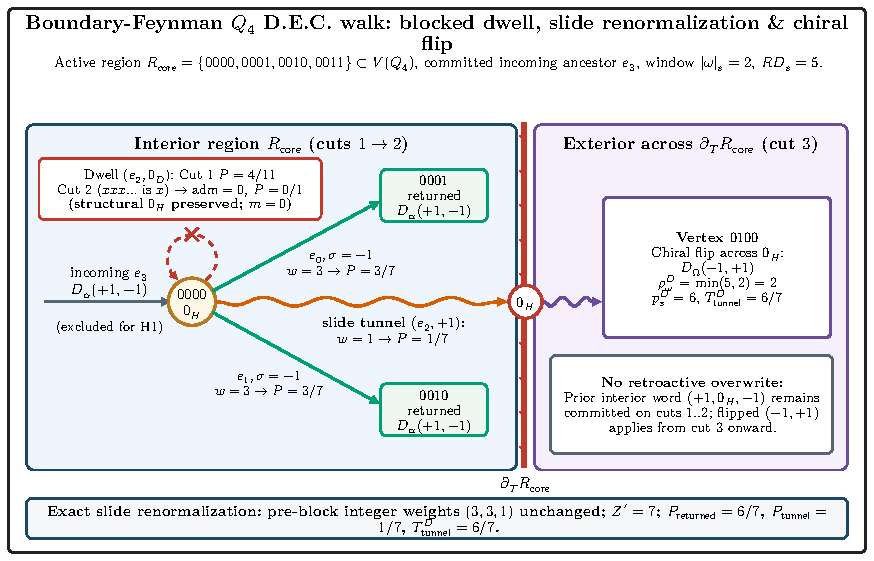
\includegraphics[width=0.92\linewidth,height=0.78\textheight,keepaspectratio]{figures/generated/dec-hinge-slide-chiral-vertex.pdf}
\caption{Boundary-Feynman $Q_4$ D.E.C. walk across $\partial_TR_{\mathrm{core}}$ (\texttt{RC-025}): live \texttt{xxxxx... is x} dwell block ($m=0$, structural $0_H$ preserved), exact slide renormalization ($Z'=7$), and post-hinge chiral flip $D_{\alpha}\to D_{\Omega}$ into vertex $0100$.}
\label{fig:manual-dec-chiral-flip-walk}
\end{figure}

\paragraph{Two-carrier Disoma Stokes encounter (\texttt{RC-026}).}
At cut $3$ (\texttt{B\_disoma|3}), declare enclosing scope
$\mathcal{B}_{12}=(\partial F_{12},\omega_{12})$ with $|\omega_{12}|=4$,
$\mathrm{RCD}_{12}=5\Rightarrow\rho^D_{\omega}=4$,
$C_3=3\Rightarrow p^D_{12}=12$, and six shared interface seats
($i_{12}=1/6$). Opposing chiralities $\chi_1=+1$ ($D_{\alpha}$ in $R_1$)
and $\chi_2=-1$ ($D_{\Omega}$ in $R_2$) yield $\Delta\chi^{\mathrm{lag}}_{12}=+2$,
$A_{12}=+1/3$, $\varphi_{12}=+4$, and $\varphi_{21}=-4$. Finite
Stokes cancels opposite oriented interface contributions in the enclosing sum,

\[
S_{\mathrm{int}}(R_1\cup R_2;\mathcal{B}_{12})=\varphi_{12}+\varphi_{21}=+4+(-4)=0,
\]

while both channel histories remain causally operative at cut $k+1$: with both
channels present, $(S_{1,k+1},S_{2,k+1})=(-4,+4)$, whereas structural
removal of $\varphi_{21}$ changes Carrier 1's realized next state to $0$.
Zero enclosing sum does not erase operative history.

\begin{figure}[H]
\centering
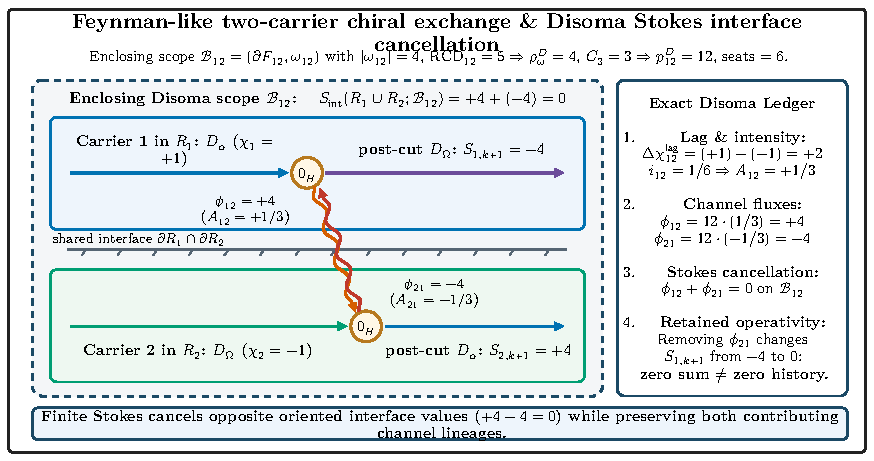
\includegraphics[width=0.92\linewidth,height=0.78\textheight,keepaspectratio]{figures/generated/chiral-flip-boundary-stokes.pdf}
\caption{Two-carrier Disoma chiral exchange across $\partial R_1\cap\partial R_2$ (\texttt{RC-026}). Opposite oriented interface fluxes cancel in $\mathcal{B}_{12}$ ($+4-4=0$) while both bound channel histories remain operative at cut $k+1$.}
\label{fig:manual-chiral-stokes-feynman}
\end{figure}

\subsection{Boundary closure and sheddic route audit}\label{manual:dec-ledger:boundary-audit}

\paragraph{Specialization.}
Declare total active pressure and closure threshold

\[
P^D=27,\qquad C_{\mathrm{close}}=24.
\]

Then exact signed closure residual and nonnegative shedding surplus are

\[
\Delta_{\mathrm{close}}=P^D-C_{\mathrm{close}}=3,\qquad X_{\mathrm{shedding}}=\max(0,\Delta_{\mathrm{close}})=3.
\]

This positive surplus matches the Dimonnanyro row, while explicit route identity and
retained-form witnesses remain separate audit obligations:

\[
1:2:9_{\mathrm{yro}}=\mathrm{Dimonnanyro}.
\]

Fixture-comparator rows record exact $\delta_3$ residuals; boundary-route rows record
boundary values and route audits separately.

\subsection{D.E.C. audit invariants}\label{manual:dec-ledger:audit-hooks}

\paragraph{Falsification invariants.}
Every valid D.E.C. ledger row carries the nine-tuple

\[
B,\quad v,\quad e,\quad v_e,\quad\sigma(e),\quad\operatorname{adm}(e;B),\quad w(e;B),\quad P(e;B),\quad\operatorname{route}(e;B),
\]

and fails audit if any of the following four invariants is broken: exact kernel
normalization over admissible rows,

\[
\sum_eP(e;B)=1,
\]

structural zero probability for zero admissibility,

\[
\operatorname{adm}(e;B)=0\Rightarrow P(e;B)=0,
\]

empty admitted optional-dwell family prior to hinge-slide renormalization,

\[
\mathrm{Adm}^0_B(e,\sigma)=\emptyset,
\]

and oriented SADAR antisymmetry across reverse channel views,

\[
\SADARop_B(C_{\bar{e}})=-\SADARop_B(C_e).
\]

Fixture-comparator rows form exact $\delta_3$ tallies, and every Tau missing-burden
row preserves integer numerator/denominator provenance

\[
\mathrm{miss}_{\tau}(K)=M_{\mathrm{miss}}(K)/M_{\mathrm{ref}}(K),
\]

with any decimal value treated strictly as a display coordinate.

\subsection{Tau missing-burden exact ratio}\label{manual:dec-ledger:tau-ratio}

\paragraph{Specialization.}
The Tau missing-burden diagnostic records exact rational provenance:

\[
\mathrm{miss}_{\tau}(K)=\frac{M_{\mathrm{miss}}(K)}{M_{\mathrm{ref}}(K)}.
\]

For the Dimonnanyro row ($1:2:9_{\mathrm{yro}}$),

\[
M_{\mathrm{miss}}=31,\qquad M_{\mathrm{ref}}=50,\qquad\mathrm{miss}_{\tau}(1:2:9_{\mathrm{yro}})=\frac{31}{50},
\]

with decimal presentation coordinate

\[
\mathrm{missing\_fraction\_display}=0.62.
\]

\begin{table}[H]
\centering
\caption{Tau missing-burden exact-ratio fields.}
\label{tab:manual-dec-tau-missing-ratio-fields}
{\footnotesize
\begin{tabular}{ll}
\toprule
field & meaning \\
\midrule
\texttt{missing\_num} & numerator $M_{\mathrm{miss}}$ \\
\texttt{missing\_den} & denominator $M_{\mathrm{ref}}$ \\
\texttt{missing\_frac\_exact} & exact ratio \\
\texttt{missing\_fraction\_display} & decimal presentation field \\
\bottomrule
\end{tabular}
}
\end{table}

\paragraph{Atomic leg and hinge role.}
Each D.E.C. row records the Hamming--1 base traversal separately from its ternary role.
Removing optional dwell sets $m=0$ in $\varepsilon0_H(0_D)^m(-\varepsilon)$
while preserving the mandatory structural hinge $0_H$---verified in exact 2-bit
SWAR arithmetic by \texttt{RC-045} (\texttt{ternary\_swar\_and\_trit\_ratio}), where
live dwell compaction burns \texttt{00} ($0_D$) while preserving \texttt{11} ($0_H$)
and polar lanes \texttt{01}/$+1$ and \texttt{10}/$-1$. A slide pool is entered only
after that hinge, kernel normalization uses already admissible support, and repeated
updates remain continuation traces until actual closure and distinct-reclosure
witnesses establish wave admission.
